% =============================================================================
% Relatorio: Atividade Simbolos I/Q (BPSK, QPSK e 16-QAM) com GNU Radio
% Padrao visual: PPGEE/UFAM (mesma identidade do modelo mestrado_ppgee)
% Normas: ABNT (NBR 14724, 10520, 6023), portugues culto, sem travessoes
% =============================================================================
\documentclass[12pt,a4paper]{article}

\usepackage[T1]{fontenc}
\usepackage[utf8]{inputenc}
\usepackage[brazil]{babel}
\usepackage{mathptmx}
\usepackage{microtype}
\usepackage{geometry}
\usepackage{xcolor}
\usepackage{fancyhdr}
\usepackage{setspace}
\usepackage{indentfirst}
\usepackage{booktabs}
\usepackage{array}
\usepackage{mdframed}
\usepackage{amsmath,amssymb}
\usepackage{graphicx}
\usepackage{float}
\usepackage{caption}
\usepackage{subcaption}
\usepackage{enumitem}
\usepackage{siunitx}
\usepackage{tikz}
\usepackage{pgfplots}
\usepackage{titlesec}
\usepackage{hyperref}
\emergencystretch=3em

\pgfplotsset{compat=1.16}
\usetikzlibrary{arrows.meta,positioning,calc,shapes.geometric}
\sisetup{output-decimal-marker={,}, group-separator={.}, group-minimum-digits=4}

\geometry{top=3cm,bottom=2.5cm,left=3cm,right=2.5cm}

\definecolor{ufamblue}{RGB}{0,51,102}
\definecolor{lightblue}{RGB}{230,240,255}
\definecolor{metabg}{RGB}{245,245,245}
\definecolor{okgreen}{RGB}{0,120,60}
\definecolor{cI}{RGB}{31,119,180}
\definecolor{cQ}{RGB}{214,95,0}

\hypersetup{
  colorlinks=true, linkcolor=ufamblue, urlcolor=ufamblue, citecolor=ufamblue,
  pdftitle={Atividade de Símbolos I/Q: BPSK, QPSK e 16-QAM no GNU Radio},
  pdfauthor={Matheus Serrão Uchôa}
}

\pagestyle{fancy}
\fancyhf{}
\rhead{\small\color{ufamblue} PPGEE/UFAM, Símbolos I/Q}
\lhead{\small\color{ufamblue} Matheus Serrão Uchôa}
\cfoot{\thepage}
\renewcommand{\headrulewidth}{0.4pt}

\titleformat{\section}{\normalfont\large\bfseries\color{ufamblue}}{\thesection}{0.8em}{\MakeUppercase}
\titleformat{\subsection}{\normalfont\normalsize\bfseries\color{ufamblue}}{\thesubsection}{0.8em}{}
\titlespacing*{\section}{0pt}{16pt}{8pt}
\titlespacing*{\subsection}{0pt}{12pt}{6pt}

\captionsetup{font=small,labelfont=bf,labelsep=colon,justification=centering}
\setlength{\parindent}{1.25cm}
\setlength{\parskip}{0pt}
\newcommand{\fonte}[1]{\par\vspace{2pt}{\small Fonte: #1}\par}
\newcommand{\sq}[1]{\ensuremath{\sqrt{#1}}}

\newcommand{\figuras}{figuras}

\begin{document}
\onehalfspacing

% -- Cabeçalho institucional (padrão PPGEE) ---------------------------------
\begin{center}
  
\includegraphics[width=2.6cm]{../mestrado_ppgee/ufam_logo.png}\\[6pt]
  \textcolor{ufamblue}{\Large\bfseries Universidade Federal do Amazonas}\\[3pt]
  \textcolor{ufamblue}{\large Programa de Pós-Graduação em Engenharia Elétrica}\\[10pt]
  \rule{\linewidth}{1.5pt}\\[6pt]
  {\LARGE\bfseries Símbolos I/Q em Modulações Digitais}\\[4pt]
  {\large\bfseries BPSK, QPSK e 16-QAM no GNU Radio Companion}\\[6pt]
  \rule{\linewidth}{1.5pt}
\end{center}

\vspace{4mm}
\begin{mdframed}[backgroundcolor=metabg,linecolor=ufamblue,linewidth=1pt,
                 innertopmargin=8pt,innerbottommargin=8pt,
                 innerleftmargin=10pt,innerrightmargin=10pt]
\begin{tabular}{@{}ll@{}}
  \textbf{Integrante da equipe:} & Matheus Serrão Uchôa \\[3pt]
  \textbf{Equipe (arquivos .grc):} & MATHEUS \\[3pt]
  \textbf{E-mail:}               & maktheus@gmail.com \\[3pt]
  \textbf{Atividade:}            & Evidências dos experimentos e questões (aula 2) \\[3pt]
  \textbf{Data:}                 & \today \\
\end{tabular}
\end{mdframed}

\vspace{6mm}
\begin{center}\textbf{\color{ufamblue}RESUMO}\end{center}
\begin{singlespace}
\small\noindent Este relatório documenta a construção, a execução e a análise de três fluxogramas do GNU Radio Companion que geram símbolos BPSK, QPSK e 16-QAM a partir de uma fonte aleatória de inteiros e de um bloco de mapeamento por tabela de símbolos. Para cada modulação, são apresentados o fluxograma, a constelação observada no plano I/Q e a saída temporal das componentes em fase (I) e em quadratura (Q). Os níveis observados confirmam a teoria: dois pontos sobre o eixo I na BPSK, quatro pontos a distância unitária da origem na QPSK e dezesseis pontos distribuídos em quatro níveis por eixo na 16-QAM, com energia média unitária após a normalização. As seis questões da atividade são respondidas com demonstrações algébricas, e a taxa de bits a \num{32000}~símbolos/s cresce de \SI{32}{kbit/s} (BPSK) para \SI{64}{kbit/s} (QPSK) e \SI{128}{kbit/s} (16-QAM).\\[4pt]
\textbf{Palavras-chave:} GNU Radio. Modulação digital. BPSK. QPSK. 16-QAM. Constelação I/Q.
\end{singlespace}

\clearpage
\tableofcontents
\clearpage

% =============================================================================
\section{Introdução}
% =============================================================================

Toda comunicação digital parte de uma sequência de bits, mas o meio físico só transporta sinais elétricos ou eletromagnéticos. A modulação digital faz a ponte entre esses dois mundos, pois associa grupos de bits a símbolos, e cada símbolo corresponde a uma forma de onda com amplitude e fase bem definidas \cite{proakis2008,haykin2008}. Nesse contexto, a representação em banda base por um número complexo, cuja parte real é a componente em fase (I) e cuja parte imaginária é a componente em quadratura (Q), permite estudar qualquer modulação linear sobre um único plano.

Diante disso, a escolha da modulação determina um compromisso entre eficiência espectral e robustez ao ruído. A BPSK transporta um bit por símbolo e é a mais robusta das três, a QPSK dobra a taxa de bits mantendo a mesma taxa de símbolos, e a 16-QAM a quadruplica, porém com pontos mais próximos entre si e, portanto, mais sensíveis ao ruído \cite{sklar2001}. Por essa razão, sistemas reais, como o Wi-Fi, alternam dinamicamente entre essas constelações conforme a qualidade do enlace.

Para observar esses efeitos de modo concreto, este trabalho utiliza o GNU Radio Companion, um ambiente de blocos para radiodefinido por software. Em cada experimento, o bloco \textit{Random Source} produz inteiros uniformemente distribuídos, o bloco \textit{Chunks to Symbols} converte cada inteiro em um símbolo complexo por consulta a uma tabela, e dois instrumentos virtuais exibem o resultado: a constelação no plano I/Q e as componentes I e Q em função do tempo.

Por fim, o relatório está organizado conforme a ordem de entrega da atividade. A Seção~\ref{sec:proc} descreve o procedimento de cada experimento, a Seção~\ref{sec:res} apresenta as nove capturas principais acompanhadas de sua interpretação, a Seção~\ref{sec:quest} responde às seis questões com os cálculos necessários, e a Seção~\ref{sec:concl} reúne as conclusões. Em todas as etapas, os valores numéricos citados foram obtidos dos dados efetivamente capturados na execução dos fluxogramas, e não digitados manualmente.

% =============================================================================
\section{Procedimento Experimental}\label{sec:proc}
% =============================================================================

\subsection{Cadeia de processamento comum}

O primeiro passo consistiu em definir a variável \texttt{samp\_rate} igual a \SI{32000}{} amostras por segundo, valor que, com um símbolo por amostra, corresponde a \num{32000}~símbolos/s. Em seguida, o bloco \textit{Random Source} foi configurado para gerar bytes no intervalo de \texttt{Minimum} igual a 0 até \texttt{Maximum}$-1$. Como o limite superior é exclusivo, o parâmetro \texttt{Maximum} é exatamente o tamanho do alfabeto de símbolos: 2, 4 e 16 nas três modulações.

Na sequência, o bloco \textit{Chunks to Symbols}, em modo \textit{Byte} para \textit{Complex} e com uma dimensão, usa cada byte recebido como índice da \textit{Symbol Table} e entrega o elemento complexo correspondente. Depois disso, um bloco \textit{Throttle} limita o fluxo à taxa de \SI{32000}{} amostras por segundo, o que torna o tempo de simulação coerente com o tempo real. Por fim, o fluxo alimenta o \textit{QT GUI Constellation Sink} e o \textit{QT GUI Time Sink}, este último configurado para entradas complexas, de modo a exibir em curvas separadas as partes real (I) e imaginária (Q).

\begin{figure}[H]
\centering
\begin{tikzpicture}[
  blk/.style={draw=ufamblue,fill=lightblue,rounded corners=2pt,minimum height=1.1cm,minimum width=2.5cm,align=center,font=\small},
  arr/.style={-{Stealth[length=2.5mm]},thick,color=ufamblue},
  node distance=0.55cm]
  \node[blk] (rs) {Random Source\\{\scriptsize Max $=M$}};
  \node[blk,right=of rs] (cs) {Chunks to\\Symbols\\{\scriptsize Symbol Table}};
  \node[blk,right=of cs,minimum width=1.9cm] (th) {Throttle\\{\scriptsize 32 kS/s}};
  \node[blk,right=of th,yshift=0.9cm,minimum width=2.2cm] (cst) {Constellation\\Sink};
  \node[blk,right=of th,yshift=-0.9cm,minimum width=2.2cm] (tms) {Time Sink\\{\scriptsize I e Q}};
  \draw[arr] (rs)--node[above,font=\scriptsize]{byte}(cs);
  \draw[arr] (cs)--node[above,font=\scriptsize]{$I+jQ$}(th);
  \draw[arr] (th.east)--++(0.3,0)|-(cst.west);
  \draw[arr] (th.east)--++(0.3,0)|-(tms.west);
\end{tikzpicture}
\caption{Cadeia de blocos comum aos três experimentos, em que $M$ vale 2 (BPSK), 4 (QPSK) e 16 (16-QAM)}
\fonte{elaborado pelo autor.}
\end{figure}

\subsection{Parâmetros específicos de cada experimento}

A Tabela~\ref{tab:param} resume o que muda de um experimento para o outro. Na BPSK, a tabela possui dois elementos reais, de modo que a componente Q permanece nula. Na QPSK, a tabela passa a ter quatro elementos complexos de módulo unitário, obtidos por divisão por \sq{2}. Já na 16-QAM, a tabela possui dezesseis elementos formados pelo produto cartesiano dos níveis $\{-3,-1,+1,+3\}$ em cada eixo, divididos por \sq{10}. Assim, apenas dois parâmetros foram alterados entre os fluxogramas, a saber \texttt{Maximum} e \texttt{Symbol Table}, enquanto o restante da cadeia permaneceu idêntico.

\begin{table}[H]
\centering\small
\caption{Parâmetros dos blocos nos três experimentos}\label{tab:param}
\begin{tabular}{@{}llp{7.2cm}@{}}
\toprule
\textbf{Modulação} & \textbf{Maximum} & \textbf{Symbol Table (índices 0, 1, \dots)}\\
\midrule
BPSK   & 2  & \texttt{[-1+0j, 1+0j]}\\
QPSK   & 4  & \texttt{[(-1-1j), (-1+1j), (1-1j), (1+1j)]/2**0.5}\\
16-QAM & 16 & dezesseis elementos \texttt{(I+jQ)/10**0.5}, com $I,Q\in\{-3,-1,+1,+3\}$ (Tabela~\ref{tab:16qam})\\
\bottomrule
\end{tabular}
\fonte{elaborado pelo autor, a partir dos arquivos \texttt{.grc} entregues.}
\end{table}

\subsection{Execução e obtenção das evidências}

Os três arquivos, \texttt{aula2\_bpsk\_MATHEUS.grc},\ \texttt{aula2\_qpsk\_MATHEUS.grc}\ e\ \texttt{aula2\_16qam\_MATHEUS.grc}, foram compilados com o utilitário \texttt{grcc} e executados com os blocos reais do GNU Radio 3.10. A partir dessa execução, foram registradas as amostras dos símbolos, das quais se extraíram os níveis de I e Q, a quantidade de pontos distintos e a energia média, resumidos na Tabela~\ref{tab:medido}. Dessa forma, as constelações e as saídas temporais da Seção~\ref{sec:res} são derivadas desses mesmos dados e podem ser reproduzidas pelos \textit{scripts} listados no Apêndice~A.

% =============================================================================
\section{Resultados e Interpretação das Saídas}\label{sec:res}
% =============================================================================

% Resultados: por modulação, quatro parágrafos (fluxo, constelação, saída temporal, interpretação).
\newcommand{\figfluxo}[2]{%
\begin{figure}[H]\centering
\includegraphics[width=\linewidth]{figuras/#1_fluxo.png}
\caption{Fluxo do GNU Radio para #2, com os parâmetros \textit{Random Source/Maximum} e \textit{Chunks to Symbols/Symbol Table}}\label{fig:#1-fluxo}
\fonte{captura de tela do GNU Radio Companion com o arquivo \texttt{.grc} entregue; o painel inferior transcreve os parâmetros lidos do arquivo.}
\end{figure}}
\newcommand{\figconst}[2]{%
\begin{figure}[H]\centering
\includegraphics[width=0.78\linewidth]{figuras/#1_constelacao.png}
\caption{Constelação #2 observada no plano I/Q}\label{fig:#1-const}
\fonte{elaborado pelo autor, a partir de 5000 símbolos produzidos pelos blocos do GNU Radio.}
\end{figure}}
\newcommand{\figtemp}[2]{%
\begin{figure}[H]\centering
\includegraphics[width=\linewidth]{figuras/#1_temporal.png}
\caption{Saída temporal das componentes I e Q da #2}\label{fig:#1-temp}
\fonte{elaborado pelo autor, a partir dos mesmos símbolos produzidos pelos blocos do GNU Radio.}
\end{figure}}

\subsection{Captura 1 a 3: BPSK}

O fluxo da BPSK, mostrado na Figura~\ref{fig:bpsk-fluxo}, liga o \textit{Random Source} com \texttt{Maximum} igual a 2 ao \textit{Chunks to Symbols} com \texttt{Symbol Table} \texttt{[-1+0j, 1+0j]}, e daí ao \textit{Throttle} e aos dois instrumentos de visualização. Como o alfabeto possui apenas dois símbolos, cada símbolo carrega um único bit. Desse modo, o fluxo é o mais simples dos três e serve de referência para as modificações posteriores.

\figfluxo{bpsk}{BPSK}

Quanto à constelação, a Figura~\ref{fig:bpsk-const} exibe somente dois pontos, em $(-1,0)$ e $(+1,0)$, ambos sobre o eixo I. Nos 5000 símbolos capturados, foram observados exatamente 2 pontos distintos, e a componente Q foi nula em todas as amostras. Por consequência, a informação da BPSK está inteiramente na fase, que vale $180^\circ$ ou $0^\circ$.

\figconst{bpsk}{BPSK}

A saída temporal da Figura~\ref{fig:bpsk-temp} confirma esse comportamento. A componente I alterna aleatoriamente entre $-1$ e $+1$, com degraus de duração múltipla de $\SI{0,03125}{ms}$, que é o período de um símbolo a \SI{32000}{símbolos\per\second}. Em contraste, a componente Q permanece constante em zero durante todo o intervalo observado.

\figtemp{bpsk}{BPSK}

Em resumo, os resultados validam as previsões: dois símbolos, amplitude unitária, energia média igual a 1 e ausência de componente em quadratura. Dessa forma, a BPSK transporta 1 bit por símbolo e, a \SI{32000}{símbolos\per\second}, resulta em \SI{32}{kbit/s}, valor que será ampliado nas modulações seguintes.

\subsection{Captura 4 a 6: QPSK}

Na QPSK, a Figura~\ref{fig:qpsk-fluxo} mostra que a topologia permaneceu a mesma e que apenas dois parâmetros mudaram: \texttt{Maximum} passou a 4 e a \texttt{Symbol Table} passou a ter quatro elementos complexos divididos por \sq{2}. Assim, cada índice de 0 a 3 corresponde a um par de bits, e o fluxo gera 2 bits por símbolo sem qualquer outra alteração na cadeia.

\figfluxo{qpsk}{QPSK}

A constelação da Figura~\ref{fig:qpsk-const} apresenta quatro pontos, um em cada quadrante, em $(\pm0{,}7071,\ \pm0{,}7071)$. A amplitude medida foi igual a 1 para os quatro pontos, de modo que todos repousam sobre a mesma circunferência de raio unitário. Isso demonstra, na prática, a eficácia da normalização por \sq{2}.

\figconst{qpsk}{QPSK}

No domínio do tempo, a Figura~\ref{fig:qpsk-temp} mostra que I e Q assumem, cada uma, apenas os valores $-0{,}7071$ e $+0{,}7071$, e que variam de forma independente uma da outra. Em outras palavras, ambos os eixos agora carregam informação, e cada um transporta um bit do par que compõe o símbolo.

\figtemp{qpsk}{QPSK}

Em síntese, a QPSK ocupou o eixo Q, que estava ocioso na BPSK, e com isso dobrou a quantidade de bits por símbolo mantendo a energia média igual a 1. Portanto, a \SI{32000}{símbolos\per\second} a taxa de bits chega a \SI{64}{kbit/s}, sem aumentar a taxa de símbolos nem a largura de banda associada.

\subsection{Captura 7 a 9: 16-QAM}

O fluxo da 16-QAM, apresentado na Figura~\ref{fig:16qam-fluxo}, utiliza \texttt{Maximum} igual a 16 e uma \texttt{Symbol Table} de dezesseis elementos, formados pelos níveis $\{-3,-1,+1,+3\}$ em cada eixo e divididos por \sq{10}. Como a tabela precisa de 16 índices, o alfabeto passa a ter $2^4$ símbolos, e cada um carrega 4 bits. A cadeia de blocos continua idêntica à das modulações anteriores.

\figfluxo{16qam}{16-QAM}

Na constelação da Figura~\ref{fig:16qam-const}, foram observados 16 pontos distintos dispostos em grade regular de $4\times4$. Os quatro níveis observados em cada eixo são $-0{,}9487$, $-0{,}3162$, $+0{,}3162$ e $+0{,}9487$, equivalentes a $\pm3/\sqrt{10}$ e $\pm1/\sqrt{10}$. Os níveis estão destacados pelas linhas tracejadas e rotulados nas bordas da figura.

\figconst{16qam}{16-QAM}

A saída temporal da Figura~\ref{fig:16qam-temp} reforça essa leitura, pois tanto I quanto Q saltam entre exatamente quatro patamares horizontais, que coincidem com os níveis identificados na constelação. Além disso, a amplitude $|s|$ assumiu três valores, $0{,}4472$, $1{,}0000$ e $1{,}3416$, o que evidencia que os símbolos não pertencem a uma única circunferência, como ocorria na QPSK.

\figtemp{16qam}{16-QAM}

Por fim, a energia média calculada sobre os 5000 símbolos capturados foi $1{,}0048$, valor muito próximo do teórico 1, e o pequeno desvio decorre apenas da frequência amostral com que cada ponto apareceu. Assim, a 16-QAM entrega 4 bits por símbolo e \SI{128}{kbit/s} a \SI{32000}{símbolos\per\second}, ao custo de pontos mais próximos entre si.

\subsection{Síntese dos valores observados}

A Tabela~\ref{tab:medido} reúne os valores extraídos diretamente dos dados capturados e a Figura~\ref{fig:comp} compara a densidade das constelações. Observa-se que o número de pontos distintos coincide com $M$ nas três modulações, que a energia média ficou em 1 e que a taxa de bits cresce com $\log_2 M$.

\begin{table}[H]
\centering\small
\caption{Valores observados nos 5000 símbolos capturados em cada modulação}\label{tab:medido}
\begin{tabular}{@{}lcccccc@{}}
\toprule
\textbf{Modulação} & \textbf{Pontos} & \textbf{Níveis em I} & \textbf{Níveis em Q} & \textbf{$|s|$ distintos} & \textbf{$E_s$ médio} & \textbf{$R_b$ (kbit/s)}\\
\midrule
BPSK   & 2  & $\pm1$ & $0$ & 1 & 1,0000 & 32\\
QPSK   & 4  & $\pm0{,}7071$ & $\pm0{,}7071$ & 1 & 1,0000 & 64\\
16-QAM & 16 & $\pm0{,}9487;\ \pm0{,}3162$ & $\pm0{,}9487;\ \pm0{,}3162$ & 3 & 1,0048 & 128\\
\bottomrule
\end{tabular}
\fonte{elaborado pelo autor, a partir de \texttt{dados/resumo.json}, gerado dos arquivos \texttt{.csv} capturados.}
\end{table}

\begin{figure}[H]
\centering
\begin{tikzpicture}
\begin{axis}[
  ybar, bar width=18pt, width=0.8\linewidth, height=5.6cm,
  ylabel={Quantidade}, symbolic x coords={BPSK,QPSK,16-QAM}, xtick=data,
  nodes near coords, ymin=0, ymax=150, enlarge x limits=0.3,
  ymajorgrids, grid style={gray!30}, tick label style={font=\small},
  legend style={at={(0.5,-0.2)},anchor=north,legend columns=-1,font=\small},
  title={Pontos observados e taxa de bits (kbit/s)}]
\addplot[fill=ufamblue!70] coordinates {(BPSK,2) (QPSK,4) (16-QAM,16)};
\addplot[fill=cQ!80] coordinates {(BPSK,32) (QPSK,64) (16-QAM,128)};
\legend{Pontos distintos observados,Taxa de bits (kbit/s)}
\end{axis}
\end{tikzpicture}
\caption{Comparação entre as três modulações a \SI{32000}{símbolos\per\second}}\label{fig:comp}
\fonte{elaborado pelo autor, com os valores da Tabela~\ref{tab:medido}.}
\end{figure}


% =============================================================================
\section{Respostas às Questões da Atividade}\label{sec:quest}
% =============================================================================

% Respostas às questões. Cada resposta segue o encadeamento: conceito, cálculo, evidência, consequência.

\subsection*{Questão 1. Qual é a diferença entre bit e símbolo?}

O bit é a menor unidade de informação, pois assume apenas um entre dois valores, 0 ou 1, e mede a quantidade de informação em escolha binária. O símbolo, por outro lado, é o elemento do alfabeto efetivamente transmitido pelo canal, isto é, uma forma de onda com amplitude e fase específicas, que no plano I/Q corresponde a um ponto da constelação. Dessa maneira, bit pertence ao domínio da informação, enquanto símbolo pertence ao domínio do sinal.

A relação entre ambos depende do tamanho do alfabeto. Em uma modulação com $M$ símbolos distintos, cada símbolo carrega $\log_2 M$ bits, de modo que BPSK ($M=2$) leva 1 bit, QPSK ($M=4$) leva 2 bits e 16-QAM ($M=16$) leva 4 bits por símbolo. Consequentemente, a taxa de bits é o produto da taxa de símbolos pelo número de bits por símbolo, $R_b = R_s \log_2 M$.

Essa distinção explica por que aumentar a ordem da modulação eleva a vazão sem exigir mais largura de banda, já que a taxa de símbolos, que governa a ocupação espectral, permanece constante. Por conseguinte, o fluxo do GNU Radio ilustra bem o conceito: o \textit{Random Source} entrega índices que representam grupos de bits, e o \textit{Chunks to Symbols} os converte em símbolos complexos.

Em síntese, o bit é aquilo que se deseja comunicar e o símbolo é o veículo físico escolhido para comunicá-lo. Portanto, a eficiência de uma modulação é medida pela quantidade de bits que cada símbolo consegue transportar sem comprometer demasiadamente a robustez ao ruído \cite{proakis2008}.

\subsection*{Questão 2. Quantos símbolos são necessários para transmitir 100 bits em BPSK e em QPSK?}

O número de símbolos necessários é obtido dividindo-se a quantidade de bits pelo número de bits por símbolo e arredondando-se para cima, ou seja, $N_s=\lceil N_b/\log_2 M\rceil$. Assim, é preciso conhecer primeiro quantos bits cada símbolo transporta em cada modulação, o que já foi estabelecido na questão anterior.

Para a BPSK, com $\log_2 2 = 1$ bit por símbolo, resulta $N_s = 100/1 = 100$ símbolos. Para a QPSK, com $\log_2 4 = 2$ bits por símbolo, resulta $N_s = 100/2 = 50$ símbolos. Como 100 é par, não há necessidade de símbolo de preenchimento em nenhum dos dois casos.

A Figura~\ref{fig:q2} confirma graficamente essa relação inversa entre bits por símbolo e quantidade de símbolos. Observa-se que dobrar o número de bits por símbolo reduz à metade o número de símbolos para a mesma mensagem, e, caso a 16-QAM fosse empregada, bastariam 25 símbolos.

Portanto, a QPSK transmite os mesmos 100 bits em metade do tempo da BPSK quando ambas operam à mesma taxa de símbolos, o que ratifica a vantagem de eficiência espectral das modulações de ordem superior.

\begin{figure}[H]
\centering
\begin{tikzpicture}
\begin{axis}[
  ybar, bar width=22pt, width=0.7\linewidth, height=5.2cm,
  ylabel={Símbolos necessários}, xlabel={Modulação},
  symbolic x coords={BPSK,QPSK,16-QAM}, xtick=data,
  nodes near coords, ymin=0, ymax=120, enlarge x limits=0.25,
  ymajorgrids, grid style={gray!30}, tick label style={font=\small},
  title={Símbolos para transmitir 100 bits}]
\addplot[fill=ufamblue!70] coordinates {(BPSK,100) (QPSK,50) (16-QAM,25)};
\end{axis}
\end{tikzpicture}
\caption{Quantidade de símbolos necessários para transmitir 100 bits}\label{fig:q2}
\fonte{elaborado pelo autor, com $N_s=\lceil 100/\log_2 M\rceil$.}
\end{figure}

\subsection*{Questão 3. O que os eixos I e Q representam? Por que Q é zero na BPSK da atividade?}

Os eixos I e Q representam as duas componentes ortogonais do sinal em banda base. O eixo I (\textit{in-phase}) é a amplitude associada à portadora em cosseno, e o eixo Q (\textit{quadrature}) é a amplitude associada à portadora em seno, defasada de $90^\circ$. Em termos matemáticos, o sinal passa-banda é $s(t)=I(t)\cos(2\pi f_c t)-Q(t)\sin(2\pi f_c t)$, e o símbolo complexo é $I+jQ$ \cite{haykin2008}.

Visto que as duas portadoras são ortogonais, podem ser moduladas de forma independente e somadas sem interferência mútua. Por isso, o plano I/Q funciona como um mapa completo do símbolo: a distância à origem é a amplitude $\sqrt{I^2+Q^2}$ e o ângulo é a fase $\arctan(Q/I)$.

Na BPSK da atividade, a \textit{Symbol Table} é \texttt{[-1+0j, 1+0j]}, de modo que a parte imaginária de ambos os símbolos é nula. Em outras palavras, a informação está codificada apenas na fase, que vale $180^\circ$ para o índice 0 e $0^\circ$ para o índice 1, e essa diferença se manifesta integralmente no sinal da componente I.

Em consequência, a constelação BPSK ocupa somente o eixo horizontal, com dois pontos em $\pm 1$, e a curva de Q no gráfico temporal permanece sobre o valor zero. O eixo Q só passa a ser utilizado a partir da QPSK, na qual o segundo bit de cada símbolo é transportado justamente pela quadratura.

\subsection*{Questão 4. Para 32.000 símbolos por segundo, qual é a taxa de bits por segundo na BPSK e na QPSK?}

A taxa de bits é obtida por $R_b = R_s \cdot \log_2 M$, em que $R_s=\num{32000}$ símbolos/s é a taxa de símbolos definida por \texttt{samp\_rate}, com um símbolo por amostra. Esse cálculo decorre diretamente da definição de símbolo como portador de $\log_2 M$ bits.

Para a BPSK, tem-se $R_b = 32000 \times \log_2 2 = 32000 \times 1 = \SI{32000}{bit\per\second} = \SI{32}{kbit/s}$. Para a QPSK, tem-se $R_b = 32000 \times \log_2 4 = 32000 \times 2 = \SI{64000}{bit\per\second} = \SI{64}{kbit/s}$. A título de comparação, a 16-QAM resultaria em $32000\times 4=\SI{128000}{bit\per\second}$.

\begin{figure}[H]
\centering
\begin{tikzpicture}
\begin{axis}[
  ybar, bar width=24pt, width=0.7\linewidth, height=5.4cm,
  ylabel={Taxa de bits (kbit/s)}, xlabel={Modulação (a \num{32000}~símbolos/s)},
  symbolic x coords={BPSK,QPSK,16-QAM}, xtick=data,
  nodes near coords, ymin=0, ymax=150, enlarge x limits=0.25,
  ymajorgrids, grid style={gray!30}, tick label style={font=\small},
  title={Taxa de bits por modulação}]
\addplot[fill=cI!80] coordinates {(BPSK,32) (QPSK,64) (16-QAM,128)};
\end{axis}
\end{tikzpicture}
\caption{Taxa de bits para taxa de símbolos fixa em \num{32000}~símbolos/s}\label{fig:q4}
\fonte{elaborado pelo autor, com $R_b=R_s\log_2 M$.}
\end{figure}

Como mostra a Figura~\ref{fig:q4}, a taxa de bits dobra da BPSK para a QPSK sem alterar a taxa de símbolos. Logo, a largura de banda ocupada permanece a mesma, e o ganho de vazão é obtido apenas à custa de uma constelação mais densa.

\subsection*{Questão 5. Parâmetros alterados para transformar o fluxo BPSK em QPSK}

Dois parâmetros foram modificados: o \texttt{Maximum} do \textit{Random Source}, que passou de 2 para 4, e a \texttt{Symbol Table} do \textit{Chunks to Symbols}, que passou de dois elementos reais para quatro elementos complexos. Os demais blocos, incluindo o \textit{Throttle} e os instrumentos de visualização, permaneceram inalterados, e isso mostra que o mapeamento é a única parte da cadeia que define a modulação.

\paragraph{(a) Por que o Maximum passou de 2 para 4.} O \textit{Random Source} gera inteiros no intervalo de \texttt{Minimum} até \texttt{Maximum}$-1$, já que o limite superior é exclusivo. Com \texttt{Maximum} igual a 2, só existem os índices 0 e 1, suficientes para a tabela da BPSK. Como a QPSK precisa de quatro símbolos, são necessários quatro índices distintos, 0, 1, 2 e 3, o que exige \texttt{Maximum} igual a 4. Se o valor permanecesse em 2, os pontos associados aos índices 2 e 3 jamais apareceriam, e a constelação exibiria apenas dois dos quatro pontos.

\paragraph{(b) Como os índices selecionam os elementos da Symbol Table.} O \textit{Chunks to Symbols}, com uma dimensão, interpreta cada byte de entrada $v$ como posição na tabela e devolve o elemento \texttt{tabela[}$v$\texttt{]}, contando a partir de zero. Assim, o índice 0 seleciona o primeiro elemento, o índice 1 o segundo, o índice 2 o terceiro e o índice 3 o quarto. Cada índice equivale também ao valor decimal de um par de bits, visto que $0=00_2$, $1=01_2$, $2=10_2$ e $3=11_2$, e isso explica a correspondência da alínea seguinte.

\paragraph{(c) Ponto $(I,Q)$ de cada índice e par de bits.} Na tabela adotada, o bit mais significativo comanda a componente I e o bit menos significativo comanda a componente Q, sendo o bit 0 mapeado para sinal negativo e o bit 1 para sinal positivo. Esse mapeamento é de Gray, pois símbolos vizinhos na constelação diferem em apenas um bit, o que minimiza o número de erros de bit causados por um erro de símbolo \cite{proakis2008}. A Tabela~\ref{tab:qpsk} apresenta o resultado, e a Figura~\ref{fig:qpsk-teo} o mostra no plano I/Q.

\begin{table}[H]
\centering\small
\caption{Mapeamento QPSK adotado, com $1/\sqrt2\approx 0{,}7071$}\label{tab:qpsk}
\begin{tabular}{@{}cccccc@{}}
\toprule
\textbf{Índice} & \textbf{Bits} & \textbf{Elemento da tabela} & \textbf{I} & \textbf{Q} & \textbf{$|s|$}\\
\midrule
0 & 00 & \texttt{(-1-1j)/2**0.5} & $-0{,}7071$ & $-0{,}7071$ & 1\\
1 & 01 & \texttt{(-1+1j)/2**0.5} & $-0{,}7071$ & $+0{,}7071$ & 1\\
2 & 10 & \texttt{(+1-1j)/2**0.5} & $+0{,}7071$ & $-0{,}7071$ & 1\\
3 & 11 & \texttt{(+1+1j)/2**0.5} & $+0{,}7071$ & $+0{,}7071$ & 1\\
\bottomrule
\end{tabular}
\fonte{elaborado pelo autor.}
\end{table}

\begin{figure}[H]
\centering
\begin{tikzpicture}[scale=2.0]
  \draw[gray!50,->] (-1.35,0)--(1.4,0) node[right,font=\small]{I};
  \draw[gray!50,->] (0,-1.35)--(0,1.4) node[above,font=\small]{Q};
  \draw[ufamblue!50,dashed] (0,0) circle (1);
  \foreach \x/\y/\b/\i in {-1/-1/00/0,-1/1/01/1,1/-1/10/2,1/1/11/3}{
    \fill[ufamblue] ({\x*0.7071},{\y*0.7071}) circle (1.6pt);
    \node[font=\scriptsize,align=center] at ({\x*0.7071+\x*0.30},{\y*0.7071+\y*0.17}) {\b\\ índice \i};
  }
  \draw[<->,okgreen,thick] (0,0)--(0.7071,0.7071) node[midway,above left,font=\scriptsize]{$|s|=1$};
\end{tikzpicture}
\caption{Constelação QPSK teórica com mapeamento de Gray e raio unitário}\label{fig:qpsk-teo}
\fonte{elaborado pelo autor.}
\end{figure}

\paragraph{(d) Por que dividir por $\sqrt2$, com demonstração.} Sem normalização, cada elemento da tabela, como $1+1j$, tem módulo $\sqrt{1^2+1^2}=\sqrt2\approx1{,}414$, de modo que a energia por símbolo seria 2. Para que todos os símbolos fiquem à distância 1 da origem, basta dividir cada um por seu próprio módulo. A demonstração para um símbolo genérico $s=(\pm1\pm j)/\sqrt2$ é
\begin{equation}
|s|^2=\left(\pm\frac{1}{\sqrt2}\right)^2+\left(\pm\frac{1}{\sqrt2}\right)^2=\frac12+\frac12=1
\quad\Rightarrow\quad |s|=1.
\end{equation}
Como os quatro símbolos diferem apenas nos sinais, que desaparecem ao se elevar ao quadrado, a conclusão vale para todos eles. Dessa forma, a QPSK normalizada tem energia média $E_s=1$ e a mesma potência da BPSK, o que permite comparar as modulações em igualdade de condições.

\paragraph{(e) Como obter amplitude $A$.} Basta multiplicar todos os elementos da tabela por $A$, ou seja, \texttt{A*[(-1-1j), (-1+1j), (1-1j), (1+1j)]/2**0.5}. Com isso, $|s|^2=A^2\left(\tfrac12+\tfrac12\right)=A^2$, logo $|s|=A$ e os símbolos passam a repousar sobre uma circunferência de raio $A$, com energia por símbolo $E_s=A^2$. De forma equivalente, a divisão por $\sqrt2$ pode ser substituída por $A/\sqrt2$ como fator comum, e os pontos ficam em $(\pm A/\sqrt2,\ \pm A/\sqrt2)$.

\subsection*{Questão 6. Sobre a configuração 16-QAM}

A 16-QAM transmite 4 bits por símbolo e distribui seus dezesseis pontos em uma grade regular de $4\times4$ sobre o plano I/Q. Nesse arranjo, tanto a amplitude quanto a fase variam entre os símbolos, e isso diferencia a modulação das anteriores, em que apenas a fase era usada. As alíneas a seguir detalham as escolhas do fluxo.

\paragraph{(a) Por que o Maximum foi alterado para 16.} Como o \textit{Random Source} gera valores de \texttt{Minimum} até \texttt{Maximum}$-1$, para obter os índices de 0 a 15, que endereçam os dezesseis elementos da tabela, é preciso \texttt{Maximum} igual a 16. Esse valor corresponde ao tamanho do alfabeto $M=2^4$, e cada índice representa um grupo de 4 bits, de $0000_2$ a $1111_2$. Valores menores deixariam símbolos sem uso, e valores maiores poderiam gerar índices sem símbolo correspondente, isto é, acessos fora da tabela.

\paragraph{(b) Como foram obtidos os 16 símbolos e a ordem adotada.} Os símbolos resultam do produto cartesiano dos quatro níveis de amplitude $\{-3,-1,+1,+3\}$ em cada eixo, o que gera $4\times4=16$ pares $(I,Q)$. Para a ordem, o índice $i=4a+b$ é formado pelos dois bits mais significativos $a$, que escolhem o nível de I, e pelos dois bits menos significativos $b$, que escolhem o nível de Q. Em cada eixo, vale o código de Gray de dois bits, $00\to-3$, $01\to-1$, $11\to+1$ e $10\to+3$, de modo que níveis adjacentes diferem em um único bit. A Tabela~\ref{tab:16qam} mostra a tabela construída, já com os valores divididos por $\sqrt{10}$, e a Figura~\ref{fig:qam-teo} a ilustra no plano I/Q.

\begin{table}[H]
\centering\footnotesize
\caption{Symbol Table da 16-QAM (ordem do índice 0 ao 15), com $1/\sqrt{10}\approx0{,}3162$}\label{tab:16qam}
\begin{tabular}{@{}cccccc@{\hspace{1.2cm}}cccccc@{}}
\toprule
\textbf{Índ.} & \textbf{Bits} & \textbf{$I$} & \textbf{$Q$} & \textbf{$I/\sqrt{10}$} & \textbf{$Q/\sqrt{10}$} &
\textbf{Índ.} & \textbf{Bits} & \textbf{$I$} & \textbf{$Q$} & \textbf{$I/\sqrt{10}$} & \textbf{$Q/\sqrt{10}$}\\
\midrule
0  & 0000 & $-3$ & $-3$ & $-0{,}949$ & $-0{,}949$ & 8  & 1000 & $+3$ & $-3$ & $+0{,}949$ & $-0{,}949$\\
1  & 0001 & $-3$ & $-1$ & $-0{,}949$ & $-0{,}316$ & 9  & 1001 & $+3$ & $-1$ & $+0{,}949$ & $-0{,}316$\\
2  & 0010 & $-3$ & $+3$ & $-0{,}949$ & $+0{,}949$ & 10 & 1010 & $+3$ & $+3$ & $+0{,}949$ & $+0{,}949$\\
3  & 0011 & $-3$ & $+1$ & $-0{,}949$ & $+0{,}316$ & 11 & 1011 & $+3$ & $+1$ & $+0{,}949$ & $+0{,}316$\\
4  & 0100 & $-1$ & $-3$ & $-0{,}316$ & $-0{,}949$ & 12 & 1100 & $+1$ & $-3$ & $+0{,}316$ & $-0{,}949$\\
5  & 0101 & $-1$ & $-1$ & $-0{,}316$ & $-0{,}316$ & 13 & 1101 & $+1$ & $-1$ & $+0{,}316$ & $-0{,}316$\\
6  & 0110 & $-1$ & $+3$ & $-0{,}316$ & $+0{,}949$ & 14 & 1110 & $+1$ & $+3$ & $+0{,}316$ & $+0{,}949$\\
7  & 0111 & $-1$ & $+1$ & $-0{,}316$ & $+0{,}316$ & 15 & 1111 & $+1$ & $+1$ & $+0{,}316$ & $+0{,}316$\\
\bottomrule
\end{tabular}
\fonte{elaborado pelo autor.}
\end{table}

\begin{figure}[H]
\centering
\begin{tikzpicture}[scale=0.95]
  \draw[gray!50,->] (-4.3,0)--(4.5,0) node[right,font=\small]{I};
  \draw[gray!50,->] (0,-4.3)--(0,4.5) node[above,font=\small]{Q};
  \foreach \v in {-3,-1,1,3}{
    \draw[gray!25] (\v,-3.8)--(\v,3.8);
    \draw[gray!25] (-3.8,\v)--(3.8,\v);
  }
  \foreach \a/\x in {00/-3,01/-1,11/1,10/3}{
    \foreach \b/\y in {00/-3,01/-1,11/1,10/3}{
      \fill[ufamblue] (\x,\y) circle (2pt);
      \node[font=\tiny,above right=-1pt] at (\x,\y) {\a\b};
    }
  }
  \foreach \v/\t in {-3/$-3$,-1/$-1$,1/$+1$,3/$+3$}{
    \node[font=\scriptsize,below] at (\v,-3.95) {\t};
    \node[font=\scriptsize,left] at (-3.95,\v) {\t};
  }
  \node[font=\small,color=ufamblue] at (0,-5.2) {Níveis em unidades de $1/\sqrt{10}$; rótulos: bits $b_3b_2b_1b_0$};
\end{tikzpicture}
\caption{Constelação 16-QAM teórica com rótulos de Gray}\label{fig:qam-teo}
\fonte{elaborado pelo autor.}
\end{figure}

\paragraph{(c) Por que dividir por $\sqrt{10}$, com demonstração.} Sem normalização, a energia média dos dezesseis símbolos não é unitária. Cada nível $\pm1$ e $\pm3$ aparece quatro vezes em cada eixo, e portanto
\begin{equation}
E[I^2]=\frac{4\cdot1+4\cdot1+4\cdot9+4\cdot9}{16}=\frac{80}{16}=5,
\qquad
E[Q^2]=5,
\end{equation}
\begin{equation}
E_s=E[I^2+Q^2]=5+5=10.
\end{equation}
Para que a energia média seja 1, divide-se cada componente por $\sqrt{E_s}=\sqrt{10}$. Isso porque a energia escala com o quadrado da amplitude, de modo que
\begin{equation}
E_s'=\frac{1}{16}\sum_{k=1}^{16}\left[\left(\frac{I_k}{\sqrt{10}}\right)^2+\left(\frac{Q_k}{\sqrt{10}}\right)^2\right]=\frac{1}{10}\cdot\frac{160}{16}=\frac{10}{10}=1.
\end{equation}
Dessa forma, a 16-QAM passa a ter a mesma energia média por símbolo que a BPSK e a QPSK normalizadas, e a comparação entre as três modulações é feita à mesma potência média.

\paragraph{(d) Por que as amplitudes não são todas iguais.} Na QPSK, os quatro pontos repousam sobre uma única circunferência, e a informação está somente na fase. Na 16-QAM, os pontos combinam dois níveis de cada eixo, e o módulo $|s|=\sqrt{(I^2+Q^2)/10}$ assume três valores distintos. Os quatro pontos de canto, com $(\pm3,\pm3)$, têm $|s|=\sqrt{18/10}\approx1{,}342$; os oito pontos de borda, com $(\pm1,\pm3)$ e $(\pm3,\pm1)$, têm $|s|=\sqrt{10/10}=1$; e os quatro pontos internos, com $(\pm1,\pm1)$, têm $|s|=\sqrt{2/10}\approx0{,}447$. A Figura~\ref{fig:aneis} resume essa distribuição.

\begin{figure}[H]
\centering
\begin{tikzpicture}
\begin{axis}[
  ybar, bar width=26pt, width=0.72\linewidth, height=5.4cm,
  ylabel={Quantidade de símbolos}, xlabel={Amplitude $|s|$},
  symbolic x coords={0{,}447,1{,}000,1{,}342}, xtick=data,
  nodes near coords, ymin=0, ymax=10, enlarge x limits=0.3,
  ymajorgrids, grid style={gray!30}, tick label style={font=\small},
  title={Anéis de amplitude da 16-QAM normalizada}]
\addplot[fill=cQ!80] coordinates {(0{,}447,4) (1{,}000,8) (1{,}342,4)};
\end{axis}
\end{tikzpicture}
\caption{Distribuição dos 16 símbolos da 16-QAM em três anéis de amplitude}\label{fig:aneis}
\fonte{elaborado pelo autor, com $|s|=\sqrt{(I^2+Q^2)/10}$.}
\end{figure}

A razão dessa diferença é que a QAM codifica informação simultaneamente em amplitude e em fase, ao passo que a QPSK usa somente a fase. Essa escolha tem um preço, pois, com a mesma energia média, a distância mínima entre pontos vizinhos cai de $\sqrt2\approx1{,}414$ na QPSK para $2/\sqrt{10}\approx0{,}632$ na 16-QAM, e a razão entre os quadrados dessas distâncias é $2/0{,}4=5$, ou cerca de $\SI{7}{dB}$. Em consequência, a 16-QAM exige relação sinal-ruído cerca de \SI{7}{dB} maior para manter a mesma probabilidade de erro de símbolo vizinho, além de requerer amplificadores lineares, por não ter envoltória constante \cite{sklar2001}.


% =============================================================================
\section{Conclusão}\label{sec:concl}
% =============================================================================

\begin{singlespace}
\noindent\hspace{1.25cm}Os três fluxogramas do GNU Radio reproduziram a teoria: a BPSK mostrou dois pontos sobre o eixo I com Q nulo, a QPSK quatro pontos a distância unitária da origem e a 16-QAM dezesseis pontos em quatro níveis por eixo. Para trocar de modulação, bastou alterar o \texttt{Maximum} e a \textit{Symbol Table}. A normalização por \sq{2} e \sq{10} igualou a energia média a 1. A \num{32000}~símbolos/s, a taxa de bits subiu de \SI{32}{kbit/s} para \SI{64}{kbit/s} e \SI{128}{kbit/s} sem mais largura de banda, mas a distância mínima caiu de $1{,}414$ para $0{,}632$, exigindo cerca de \SI{7}{dB} a mais de relação sinal-ruído na 16-QAM. Assim, a escolha da modulação equilibra vazão e robustez.
\end{singlespace}


% =============================================================================
\begin{thebibliography}{9}
\addcontentsline{toc}{section}{Referências}
\renewcommand{\refname}{REFERÊNCIAS}
\bibitem{haykin2008} HAYKIN, S.; MOHER, M. \textbf{Sistemas de comunicação}. 5. ed. Porto Alegre: Bookman, 2011.
\bibitem{proakis2008} PROAKIS, J. G.; SALEHI, M. \textbf{Digital communications}. 5. ed. New York: McGraw-Hill, 2008.
\bibitem{sklar2001} SKLAR, B. \textbf{Digital communications: fundamentals and applications}. 2. ed. Upper Saddle River: Prentice Hall, 2001.
\bibitem{lathi2009} LATHI, B. P.; DING, Z. \textbf{Modern digital and analog communication systems}. 4. ed. New York: Oxford University Press, 2009.
\end{thebibliography}

\clearpage
\section*{Apêndice A: Rastreabilidade das evidências}
\addcontentsline{toc}{section}{Apêndice A: Rastreabilidade das evidências}

Os três arquivos, \texttt{aula2\_bpsk\_MATHEUS.grc},\ \texttt{aula2\_qpsk\_MATHEUS.grc}\ e\ \texttt{aula2\_16qam\_MATHEUS.grc}, acompanham este relatório e compilam com o utilitário \texttt{grcc} do GNU Radio 3.10.9. Os valores da Tabela~\ref{tab:medido} foram calculados a partir de 5000 símbolos por modulação, obtidos pela execução dos mesmos blocos \textit{Random Source} e \textit{Chunks to Symbols}, com os mesmos parâmetros, ligados a um \textit{Vector Sink} em lugar dos instrumentos gráficos.

Quanto à origem das figuras, as capturas de fluxo são imagens reais do GNU Radio Companion abrindo cada arquivo \texttt{.grc}, acrescidas de um painel de texto com os parâmetros exatos, porque o aplicativo trunca a \textit{Symbol Table} dentro do bloco. As constelações e as saídas temporais da Seção~\ref{sec:res} foram redesenhadas com a biblioteca \textit{matplotlib} a partir dos dados capturados, de modo a incluir título, eixos, legendas e a identificação dos níveis. Para que não restem dúvidas sobre o comportamento dos instrumentos originais, o Apêndice B traz capturas reais das janelas dos \textit{QT GUI Sinks}.

Os \textit{scripts} que geram os arquivos \texttt{.grc}, executam a captura e produzem as figuras estão na pasta \texttt{scripts} do projeto, o que permite reproduzir todos os resultados. Ressalva-se que o GNU Radio Companion rotula o bloco \textit{Throttle} como \textit{old} (captura da Figura~\ref{fig:bpsk-fluxo}) e que o \texttt{grcc} emite um aviso de descontinuação, mas o bloco permanece funcional para o propósito desta atividade, que é limitar a taxa de amostras em \SI{32000}{} por segundo.

\section*{Apêndice B: Capturas reais dos QT GUI Sinks}
\addcontentsline{toc}{section}{Apêndice B: Capturas reais dos QT GUI Sinks}

As Figuras~\ref{fig:qt-bpsk} a~\ref{fig:qt-16qam} mostram as janelas dos instrumentos do próprio GNU Radio durante a execução dos três fluxogramas. Nelas, os rótulos de eixo são os padrões do aplicativo (\textit{In-phase}, \textit{Quadrature} e \textit{Time}), e o \textit{Time Sink} liga as amostras por segmentos de reta, o que difere dos degraus das figuras redesenhadas. A sequência aleatória dessa execução é independente da usada nos arquivos \texttt{.csv}.

\begin{figure}[H]\centering
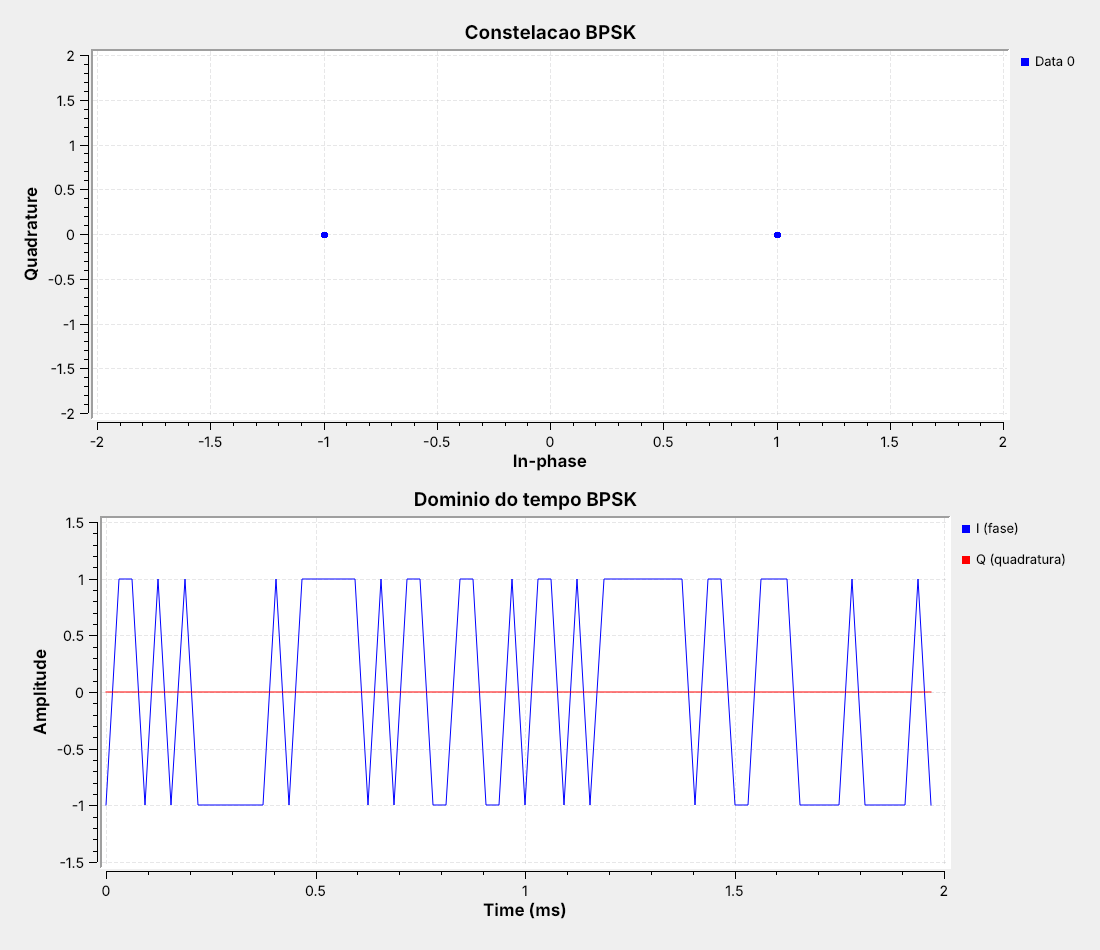
\includegraphics[width=0.78\linewidth]{figuras/extra_bpsk_qtgui_real.png}
\caption{Janela real dos instrumentos na BPSK}\label{fig:qt-bpsk}
\fonte{captura de tela da execução do fluxograma \texttt{aula2\_bpsk\_MATHEUS.grc}.}
\end{figure}
\begin{figure}[H]\centering
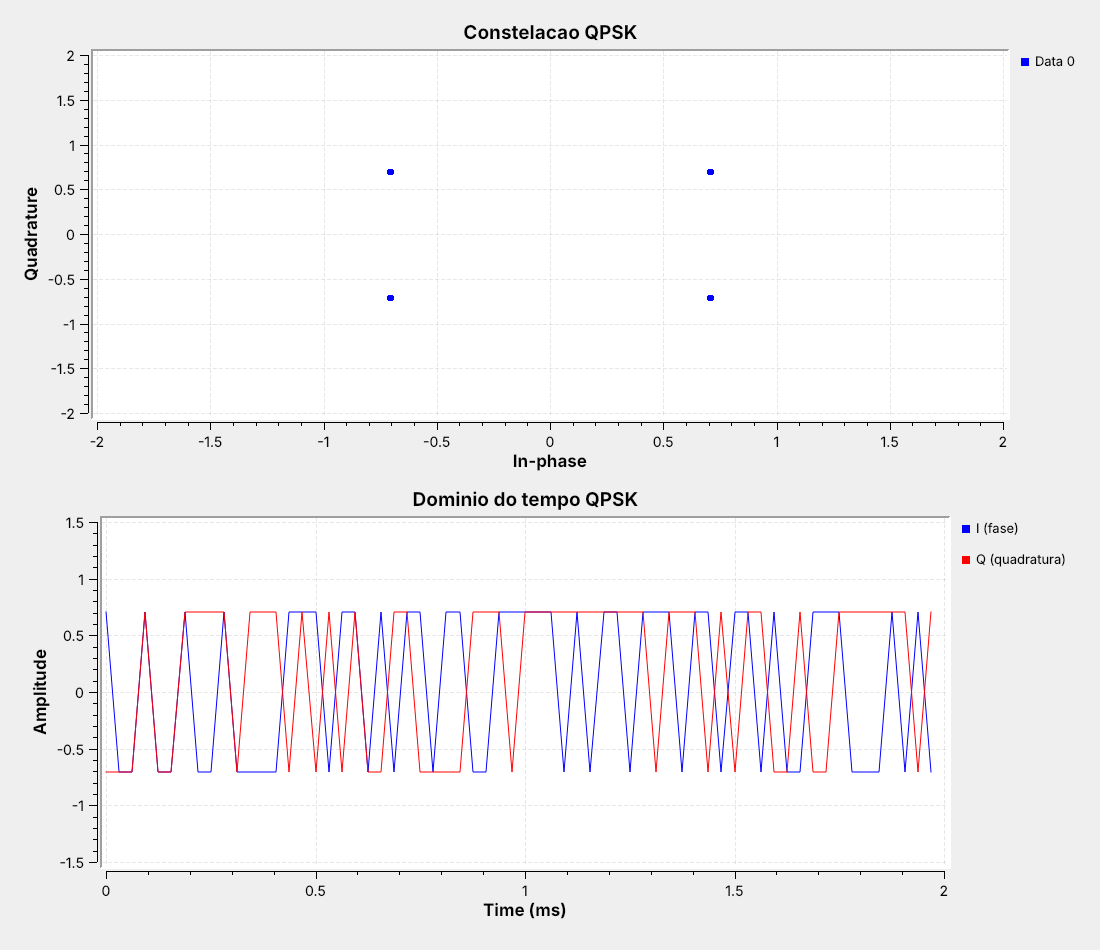
\includegraphics[width=0.78\linewidth]{figuras/extra_qpsk_qtgui_real.png}
\caption{Janela real dos instrumentos na QPSK}\label{fig:qt-qpsk}
\fonte{captura de tela da execução do fluxograma \texttt{aula2\_qpsk\_MATHEUS.grc}.}
\end{figure}
\begin{figure}[H]\centering
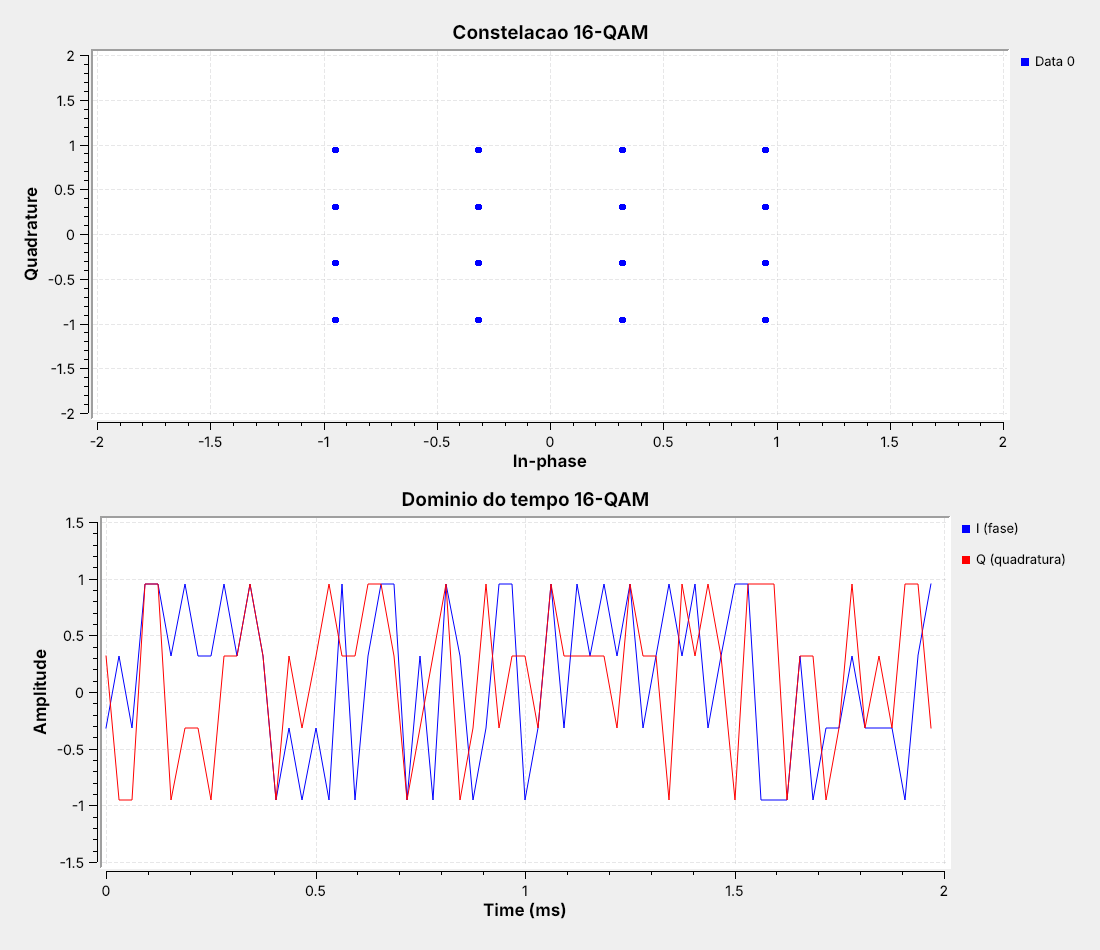
\includegraphics[width=0.78\linewidth]{figuras/extra_16qam_qtgui_real.png}
\caption{Janela real dos instrumentos na 16-QAM}\label{fig:qt-16qam}
\fonte{captura de tela da execução do fluxograma \texttt{aula2\_16qam\_MATHEUS.grc}.}
\end{figure}


\end{document}
